\section{Experimental Results: Comparison and Improvement of Static Analysis Tools}

Our primary experimental results are a set of comparisons of tools using our method, for three languages: Solidity (the most popular language for smart contracts), Java, and Python.  We also use these results to answer a set of research questions that consider the utility of our method:

\begin{itemize}
\item {\bf RQ1:}  Does our approach produce actionable results?  That is, do raw mutation kills serve to distinguish tools from each other, or are all tools similar in terms of mutation detection capability?
\item {\bf RQ2:}  Does our approach provide additional information beyond simply counting findings for the original, un-mutated analyzed code?  Do \emph{ratios} differ between programs, or does the number of mutants killed simply reflect the ``verbosity'' of each tool?
\item {\bf RQ3:}  Do the rankings that raw kills and ratios establish agree with other sources of information about the effectiveness of the evaluated tools?  Can we confirm results from other evaluation methods, or informal opinion?
\item {\bf RQ4:}  Do individual mutants, prioritized for ease of examination, allow us to identify classes of faults that different tools are good at/bad at?  Can we extend this information to improve tools by addressing identified weaknesses?
  \end{itemize}

In particular, we consider {\bf RQ2} to be of critical importance; if the mutant ratios for tools differ, then this is clear evidence that our hypothesis that the tendency of mutants to be faults, and to expect that mutated code will, by a sound and precise tool, be flagged as problematic more often than non-mutated code, holds.  This expectation that (some subset of the) mutants can serve as proxies for real, detectable faults is the core concept of our approach.
  
\subsection{Solidity Smart Contract Tools}

\subsubsection{Smart Contracts and Smart Contract Static Analysis}

Smart contracts are autonomous code instruments, usually operating on a blockchain, that often have critical responsibilities such as facilitating and verifying (large) financial services transactions, tracking high-value physical goods or intellectual property, or even controlling ``decentralized organizations'' with multifarious aspects.  Security and correctness are thus critical in the smart contract domain, and static analysis is a key way to ensure allocation of high-value resources is not compromised.  The most popular smart contract platform, by far, is the Ethereum blockchain, and the Solidity smart contract language \cite{buterin2013whitepaper,wood2014yellow}; the Ethereum cryptocurrency has a market capitalization as we write of over \$15 billion dollars, largely fueled by interest in the smart contract functionality.  Ethereum contracts have been the targets of widely publicized attacks, with large financial consequences  \cite{spank,DAO}.   A recent paper examining results from 23 professional security audits of Solidity contracts argues that effective static analysis is a major key to avoiding such disasters in the future \cite{FC20}.

\subsubsection{Static Analysis Tools Compared}

We analyzed three well-known tools for static analysis of Solidity smart contracts: Slither \cite{slither}, SmartCheck \cite{smartcheck}, and Securify \cite{Securify}. 

\subsubsection{Smart Contract Selection}

We could have used a set of high-transaction contracts, or known-important contracts to validate our approach.  However, we knew that one of our goals in the Solidity experiments was to actually improve a mutation analysis tool, and the developers of the static analysis tools use exactly such benchmarks to validate their tools.  Basing our improvements on mutants of the contracts used for evaluation of proposed detectors would introduce a serious bias in our favor: we would be more likely to produce detectors that would have true positives and few false positives on the benchmark contracts.  We therefore instead selected 100 random contracts for which EtherScan (\url{https://etherscan.io/}) has source code, and used this (quite arbitrary) set of contracts from the actual blockchain to compare tools and identify opportunities for improvement.

\subsubsection{Analysis Results}

\begin{figure}
  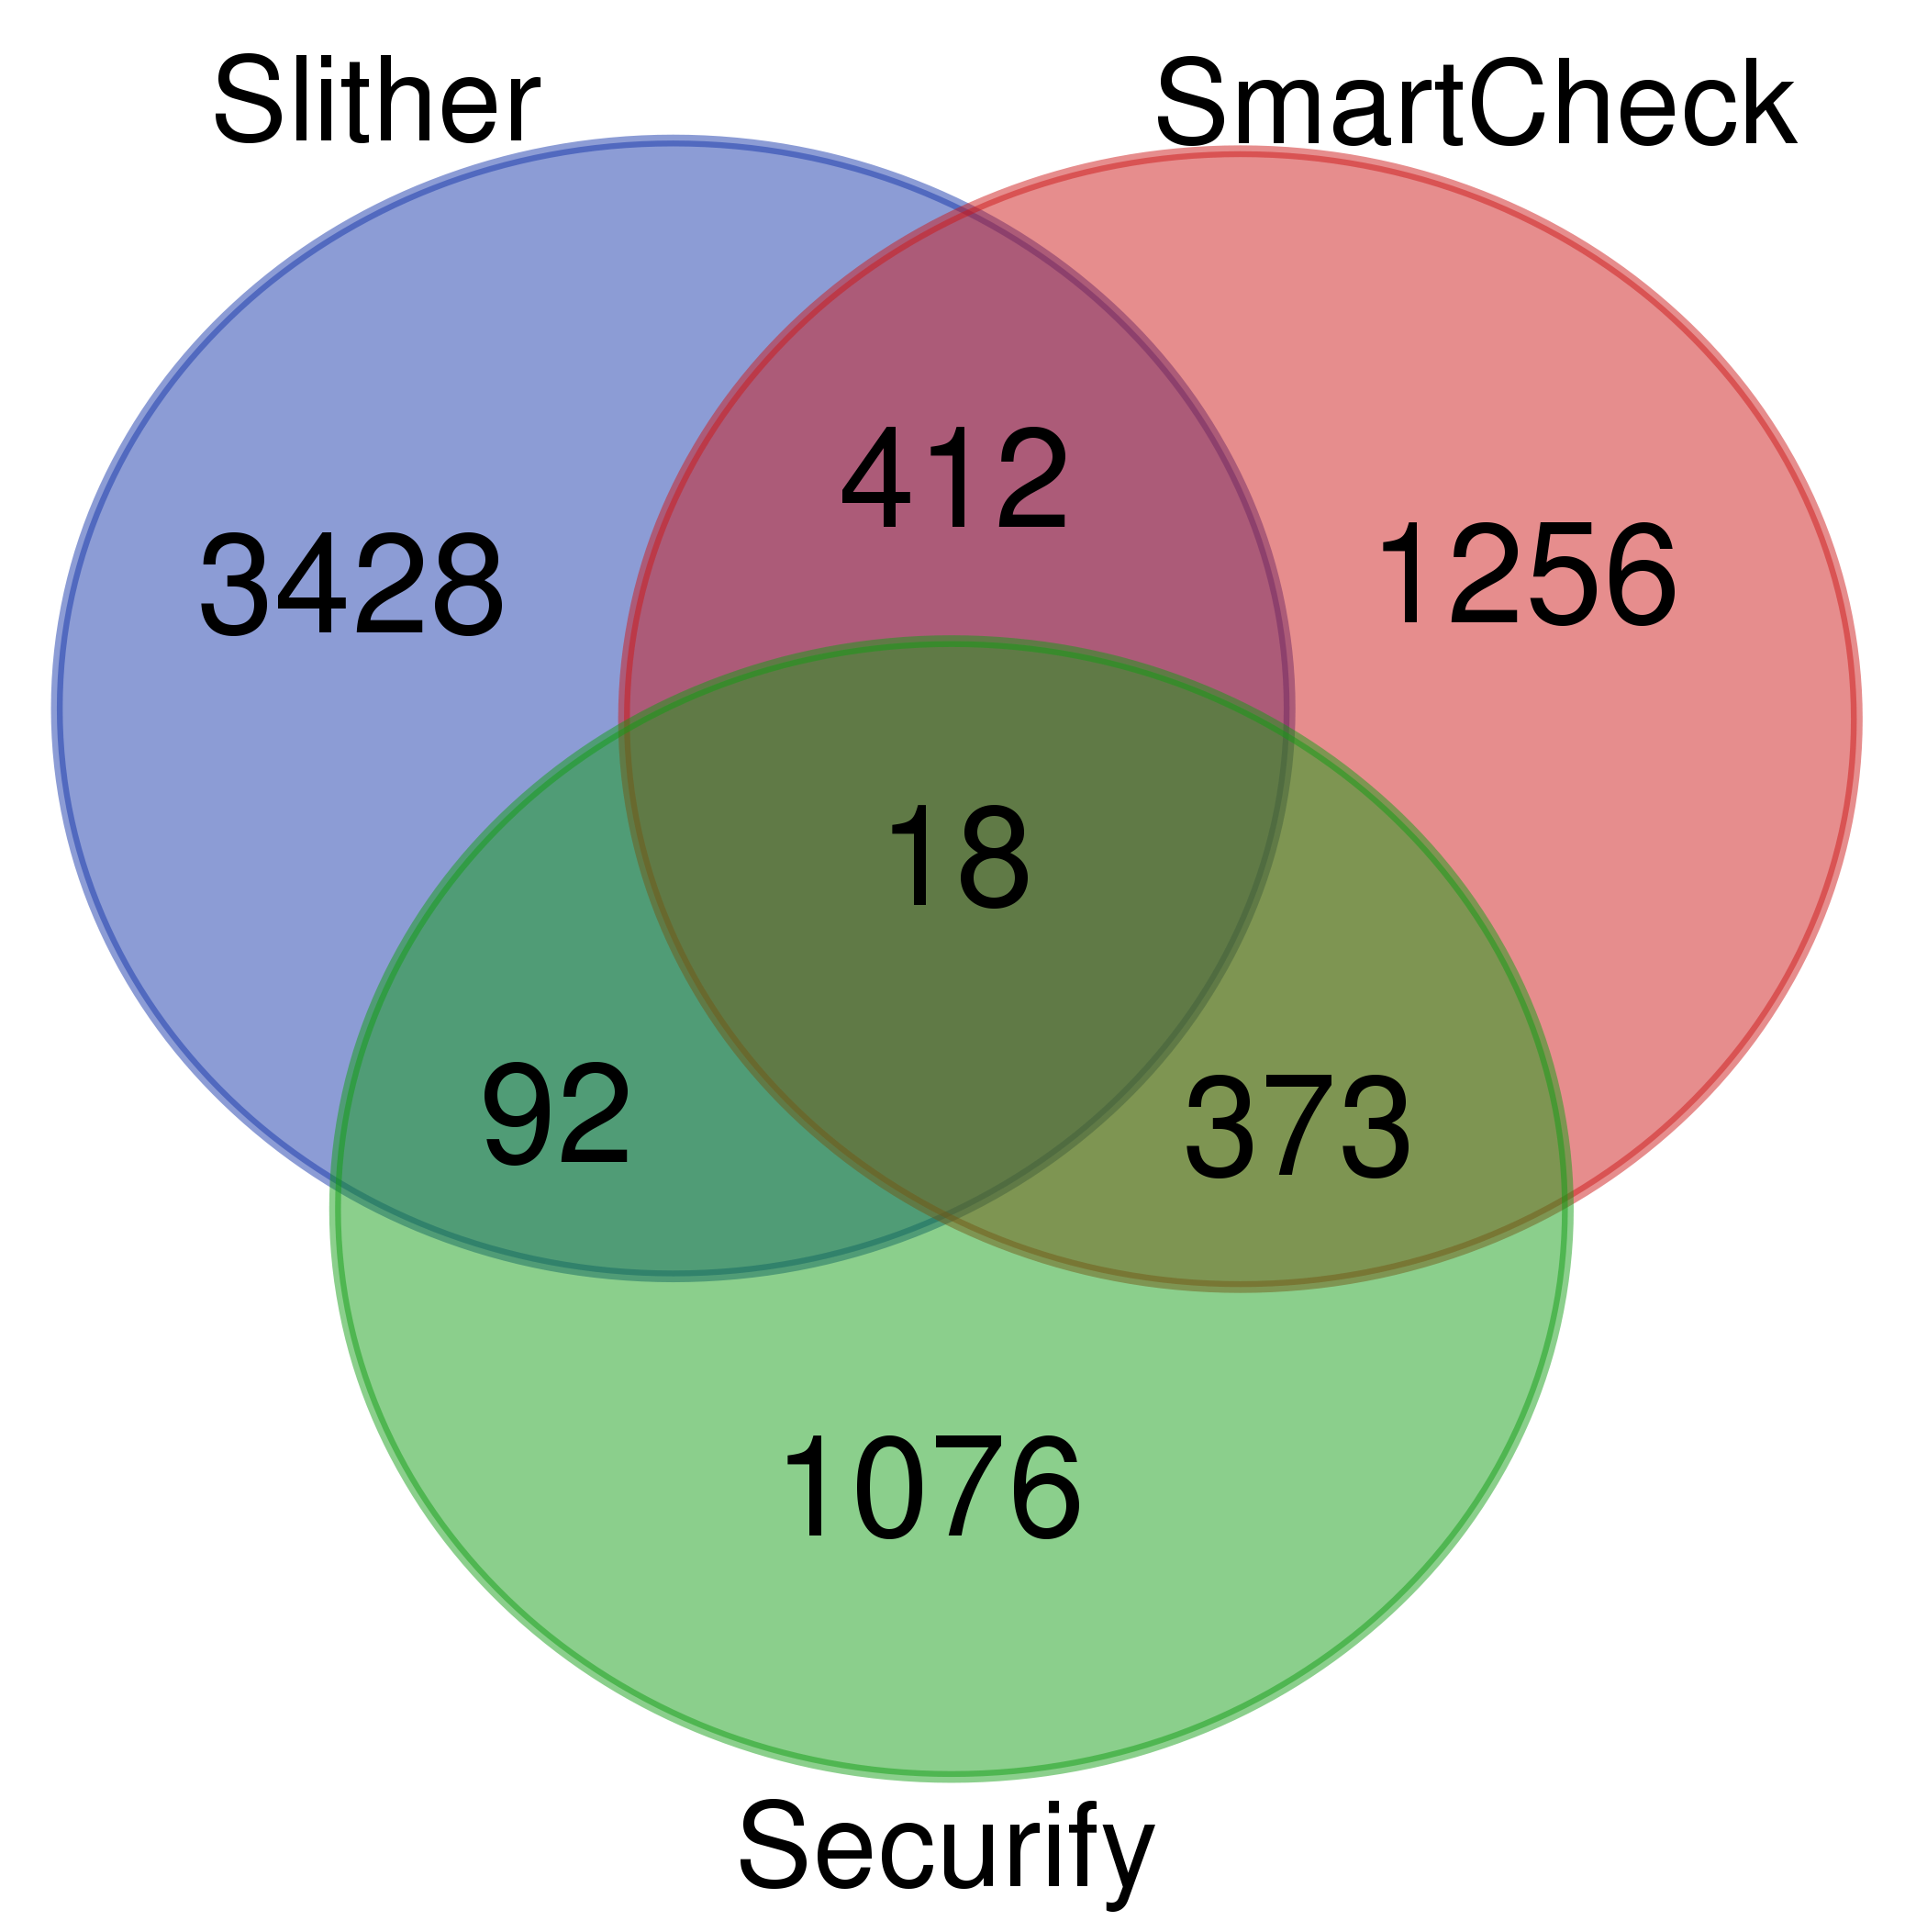
\includegraphics[width=\columnwidth]{solidity.png}
  \caption{Mutants killed by Solidity static analysis tools.}
  \label{fig:solidityvenn}
\end{figure}

\begin{table}
  \begin{tabular}{l|r|r|r|r|r}
    & \multicolumn{2}{|c|}{Findings} & \multicolumn{2}{|c|}{Mutation Score}  & Mutant \\
    Tool & Mean & Median & Mean & Median & Ratio\\
    \hline
    \hline
    Slither & 2.37 & 1.0 & 0.09 & 0.09 & 0.038 \\
    \hline
    SmartCheck & 1.89 & 1.0 & 0.05 & 0.05 & 0.026 \\
    \hline
    Securify & 24.65 & 17.0 & 0.03 & 0.02 &  0.001 \\
    \hline
  \end{tabular}
  \caption{Solidity tools: number of findings and mutation scores over all contracts.}
  \label{tab:scoresolidity}
\end{table}

\begin{table}
  \begin{tabular}{l|r|r|r|r|r}
    & & \multicolumn{2}{|c|}{} & \multicolumn{2}{|c}{Clean For All (3)} \\
    & \# Clean & \multicolumn{2}{|c|}{Mutation Score} &  \multicolumn{2}{|c}{Mutation Score}\\
    Tool & Contracts & Mean & Median & Mean & Median\\
    \hline
    \hline
    Slither & 39 & 0.11 & 0.11 & 0.09 & 0.09 \\
    \hline
    SmartCheck & 27 & 0.03 & 0.01 & 0.03 & 0.00 \\
    \hline
    Securify & 5 & 0.00 & 0.00 & 0.00 & 0.00 \\
    \hline
  \end{tabular}
  \caption{Solidity tools: clean contract counts and mutation scores.}
  \label{tab:cleansolidity}
\end{table}


Figure \ref{fig:solidityvenn} shows the mutants killed by the Solidity analysis tools.  Tables \ref{tab:scoresolidity} and \ref{tab:cleansolidity} provide numeric details of the results, including the \emph{ratio} for each tool, adjusting its mutation scores by its' general tendency to produce findings.  First, a user examining these results would suspect that Slither and SmartCheck are both useful tools, and should likely both be applied in a high-risk security-sensitive context like smart contract development.  Second, a user might suspect that the large number of findings produced, and smaller number of mutants killed, for Securify, mean that including Securify in the static analysis tool stable is a more difficult decision.  On the one hand, Securify does detect nearly as many mutants it alone can identify as SmartCheck.  The large number of findings, and very bad mutant ratio, however, lead us to suspect that many of these ``detected'' mutants are false positives (or, at least, that the problem is not the one Securify identifies).  Extracting the signal from Securify's noise will be difficult.  We also note that while running Slither and SmartCheck on all 46,769 valid mutants was relatively quick (it took about 8 days sequential compute time for Slither and 3 days for SmartCheck), Securify often required many hours to analyze a mutant, and frequently required a few days to analyze a mutant; the full analysis required over three months of compute time.

We first compare the two tools that performed best.  Slither detected 2.37 mean issues over the 100 contracts, and found 39 contracts free of all issues.  Slither had a mean mutation score of 0.09 over all contracts, and 0.11 over clean (according to Slither) contracts.  SmartCheck detected 1.89 mean issues over the 100 contracts, but only found 27 contracts free of all issues.  The mean issue counts for the tools were not statistically significantly different ($p=0.34$).  SmartCheck had a mean mutation score of 0.05 over all contracts, and 0.03 over clean (according to SmartCheck) contracts.  The ratio between mean issues (Slither / SmartCheck) is 1.25, and the ratio of numbers of clean contracts is similar (1.44).  The mutation score ratio, however, is 1.8, suggesting that Slither is not out-scoring SmartCheck \emph{only} because it produces more false positives.  Slither detects 3,520 mutants not detected by SmartCheck, while SmartCheck only detects 1,629 mutants not detected by Slither (of these, 1,256 were also not detected by Securify) .  Over the 7 contracts that both tools mark as clean, Slither has a mean mutation score of 0.08, and SmartCheck has a mean mutation score of 0.03; the difference, even with only 7 contracts, is statistically significant by paired Wilcoxon test, at $p=0.03$.

Securify was an outlier, compared to the other tools.  First, while running Slither and SmartCheck on all 46,769 valid mutants was relatively quick, Securify often required hours to analyze a contract; the full analysis required over a month.  Second, Securify identified a mean of 24.65 issues on the un-mutated contracts, with a median of 17 issues found; this was a significant difference in issue counts from either other tool, with $p<1.0^{-15}$ in both cases.  Despite this huge number of non-informational warnings for the original contracts, the mean mutation score was even worse than for SmartCheck, 0.03.  For contracts where Securify found no issues in the original contract, it \emph{never} detected any mutants. Securify, however, did detect 1,449 mutants not detected by Slither, 1,076 of which were not detected by SmartCheck.  On the other hand, given the ratio of issue counts compared to both tools is over 10.0, it is fairly likely many of these \emph{are} false positives, despite the probability mutants are actual faults.

Our recommendation, based on mutation analysis results, is that smart contract analysis should at least use both Slither and SmartCheck, perhaps applying only Slither until it reports no interesting issues.  Securify does offer a substantial non-overlapping set of issues reported, however, but produces a very large number of false positives.  Available human resources and total number of issues produced (as well as high runtime) might justify not using Securify in some cases.

\subsubsection{Improving Slither {\bf (RQ 4)}}

Based on the differential mutation analysis, we identified three low-hanging fruit to improve the performance of Slither.  The process was simple.  First, we produced a list of all mutants killed by either SmartCheck or Securify, but not killed by Slither.  We then applied the prioritization method based on the FPF algorithm and the distance metric described in Section \ref{sec:prioritizing}, and examined the mutants in rank order.  Many of the mutants were difficult to identify as true or false positives, absent context.  Some opportunities for enhancement were clear, but seemed likely to require considerable effort to implement without producing a large number of false positives.  For example, Securify often detected when an ERC20 token contract's guard preventing making the special 0x0 address the owner of a contract was removed, and issued the error {\tt Violation for MissingInputValidation}. Detecting such missing guards is probably useful, but formulating a way to do it without producing false positives is non-trivial.  We wanted to show that mutants could identify \emph{useful} but \emph{easy to implement} missing detectors.  Examining the first few mutants, we identified three such, based on mutants killed by either SmartCheck or Securify, or both:

\begin{figure*}
\begin{code}
  0x598ab825d607ace3b00d8714c0a141c7ae2e6822\_Vault.mutant.275.sol:
  424contracts/0x598ab825d607ace3b00d8714c0a141c7ae2e6822\_Vault.sol:249
        if (!p.recipient.send(p.amount)) \{  // Make the payment
 ==>          if (true) \{  // Make the payment
        if (true) \{  // Make the payment
      \end{code}
      \caption{Mutant showing {\bf Boolean constant misuse}.}
      \label{fig:boolean}
    \end{figure*}

    \begin{figure*}
\begin{code}
  0x968815CD73647C3af02a740a2438D6f8219e7534\_TTPresale.mutant.311.sol:
  424contracts/0x968815CD73647C3af02a740a2438D6f8219e7534\_TTPresale.sol:175
        require(nextDiscountTTMTokenId6 >= 361 \&\& nextDiscountTTMTokenId6 <= 391);
 ==>  ...361...==>...0...
        require(nextDiscountTTMTokenId6 >= 0 \&\& nextDiscountTTMTokenId6 <= 391);
      \end{code}
      \caption{Mutant showing {\bf Type-based tautologies}.}
      \label{fig:tautology}      
\end{figure*}

\begin{figure*}
\begin{code}
  0x534ccee849a688581d1b0c65e7ff317ed10c5ed3\_NametagToken.mutant.480.sol:
  424contracts/0x534ccee849a688581d1b0c65e7ff317ed10c5ed3\_NametagToken.sol:650
        byte char = byte(bytes32(uint(x) * 2 ** (8 * j)));
 ==>  ...*...==>.../...
        byte char = byte(bytes32(uint(x) * 2 ** (8 / j)));
      \end{code}
      \caption{Mutant showing {\bf Loss of precision due to divide before multiply}.}
      \label{fig:divmul}            
      \end{figure*}

\begin{enumerate}
\item {\bf Boolean constant misuse:}  This detector flags code like {\tt if (true)} or {\tt g(b || true)} (where {\tt g} is a function that takes a Boolean input).  Constant-valued conditionals tend to indicate debugging efforts that have persisted into production code, or other faults; there are almost no circumstances where a conditional should not vary with state or input.  This detector is actually split into two detectors, one for this serious issue, and an informational/stylistic detector that notes that code such as {\tt if (x == true)}, while semantically harmless, is difficult to read.  This problem was easily identified from cases such as the mutant in Figure \ref{fig:boolean}, killed by SmartCheck but not Slither:

\item {\bf Type-based tautologies:}  A type-based tautology is again a case where a Boolean expression has a constant value, but this is not due to misuse of a Boolean constant, but is instead due to the \emph{types} in a comparison.  For example, if {\tt x} is an unsigned integer type, the comparison {\tt x >= 0} is always true and {\tt x < 0} is always false.  This detector is a generalization of the SmartCheck detector \url{https://github.com/smartdec/smartcheck/blob/master/rule\_descriptions/SOLIDITY\_UINT\_CANT\_BE\_NEGATIVE/description\_en.html}, modified to actually compute the ranges of types and identify more general instances of tautological comparisons, e.g. {\tt y < 512} where {\tt y}'s type is {\tt int8}.  Again, the problem was easily identified by mutants killed by SmartCheck but not Slither such as the one in Figure \ref{fig:tautology}.

\item {\bf Loss of precision due to divide before multiply:}  Solidity only supports integer types.  This means that performing division before multiplication can introduce rounding that is not present when the multiplication is performed first.  This is a fairly important problem, given the frequency with which Solidity code performs financial calculations where maximum precision is desired.  SmartCheck provides a detector for such precision losses \url{https://github.com/smartdec/smartcheck/blob/master/rule\_descriptions/SOLIDITY\_DIV\_MUL/description\_en.html}, which enabled it to detect mutants such as the one shown in Figure\ref{fig:divmul}.
\end{enumerate}      

All three of these detectors were submitted as PRs, vetted over an internal benchmark set of contracts used by the Slither developers to evaluate new detectors, and accepted for release in the public version of Slither.  All three detectors produce some true positives (actual problems, though not always exploitable) in benchmark contracts, have acceptably low false positive rates, and were deemed valuable enough to include as non-informational (medium severity) detectors.  The first mutants in prioritized rank exhibiting the issues, shown above, were the 2nd, 9th, and 12th non-statement-deletion mutants ranked for SmartCheck, out of over 800 such mutants.  Using our prioritization, it was possible to identify these issues by examining fewer than 20 unkilled mutants.  Without prioritization, on average a developer would have to look at more than 200, 80, and 400 mutants, respectively, to find instances of these problems.  

There were 92 separately ranked statement deletion mutants also.  These, however, could all be ignored, as they were almost entirely duplicates related to the missing-return statement detector.  If this detector were not already present as a private Slither detector, it would also be a good candidate for addition to the tool.  Our three submitted detectors were not present as private detectors, and only one (the type-based tautology detector) had even been identified, via a GitHub issue, as a potential improvement (and only in the private version of Slither).  

Examining the first 100 mutants in the unprioritized lists for SmartCheck and Securify, ordered by contract ID and mutant number (roughly source line mutated) we were unable to identify \emph{any} obviously interesting mutants.  The majority of cases involved either the missing return problem or replacing {\tt msg.sender} with {\tt tx.origin}; Slither has a detector for misuses of {\tt tx.origin}, and we believe (but are not sure) that almost all of these are due to intentional behavior: SmartCheck and Securify tend to identify most uses of {\tt tx.origin} as incorrect, while Slither has a more selective rule intended to avoid false positives.

It is hard to scale our efforts here to a larger experiment, since writing and submitting changes to static analysis tools is always going to be a fairly onerous task, but we believe that our successful addition of new detectors, and the ease of identifying good candidate detectors using mutant prioritization supports a limited affirmative answer to {\bf RQ4}.



\subsection{Java Tools}
